\documentclass[10pt] {article}
\usepackage{fullpage}
\usepackage{amssymb}
\usepackage{graphicx}
\usepackage{float}
\usepackage{amsthm}
\usepackage{hyperref}
\usepackage{amsmath}
\renewcommand\qedsymbol{$\blacksquare$}

\title{Homework 5 }
\author{Ricky Hempel}
\begin{document}
\maketitle
\begin{center}
Chapter 2:
Exercises: 2.5 (state diagrams, brief descriptions),
2.7acd (algorithmic descriptions only),
2.10-2.12, 2.16, 2.17
\end{center}
\begin{enumerate}
\item[2.5] (a.)
\begin{figure}[H]
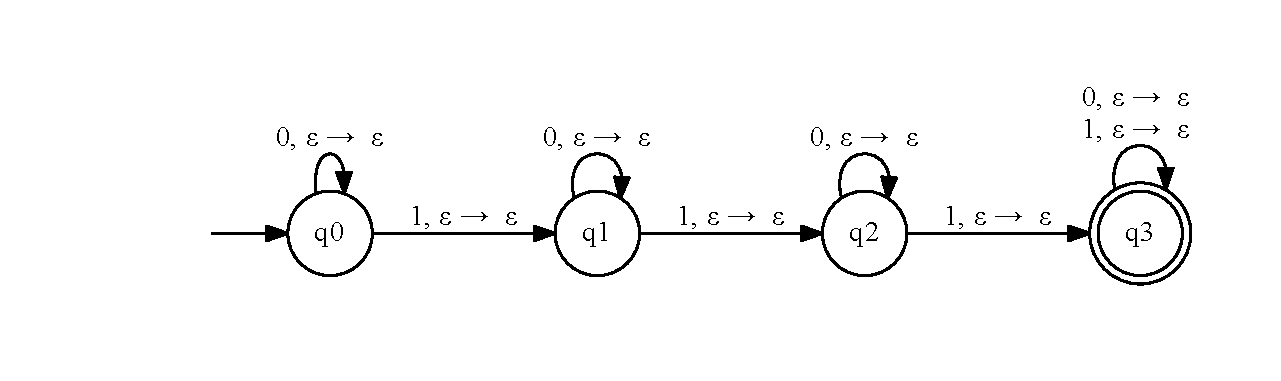
\includegraphics[width=0.9\textwidth]{a25.pdf}
\caption{The PDA for $L=\{w \mid$ w contains at least three 1s $\}$.}
\label{1}
\end{figure}
Brief Description: In this PDA we loop and do noting to the stack when we see a zero. When we see an one we transition and do nothing to the stack. After we see  three ones we loop on every symbol we see after, doing nothing to the stack, and accept.    \\
(b.)  
\begin{figure}[H]
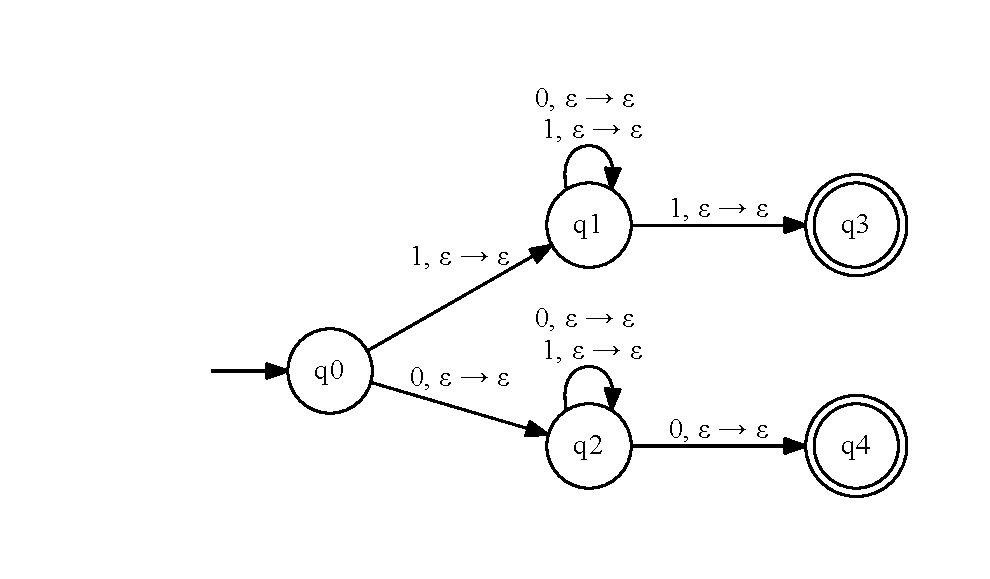
\includegraphics[width=0.7\textwidth]{b25.pdf}
\caption{The PDA for $L=\{w \mid$ w starts and ends with the same symbol $\}$.}
\label{2}
\end{figure}
Brief Description: In this PDA we go into two different machines.If we see an 1 we non-deterministicly guess if the ending symbol is the same as the is the starting symbol if it is we accept. The second machine,if we see an 0 we non-deterministicly guess if the ending symbol is the same as the is the starting symbol if it is we accept. While this is going on we do nothing to the stack.\\
(c.) 
\begin{figure}[H]
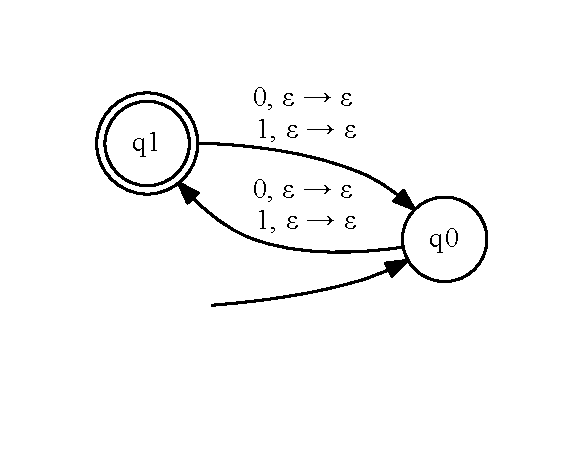
\includegraphics[width=0.5\textwidth]{c25.pdf}
\caption{The PDA for $L=\{w \mid$ w the length of w is odd $\}$.}
\label{3}
\end{figure}
Brief Description: In this PDA we transition back and forth between two states every time we see a symbol, and accept when the number of symbols is odd. While this is going on we do nothing to the stack.\\
(d.)
\begin{figure}[H]
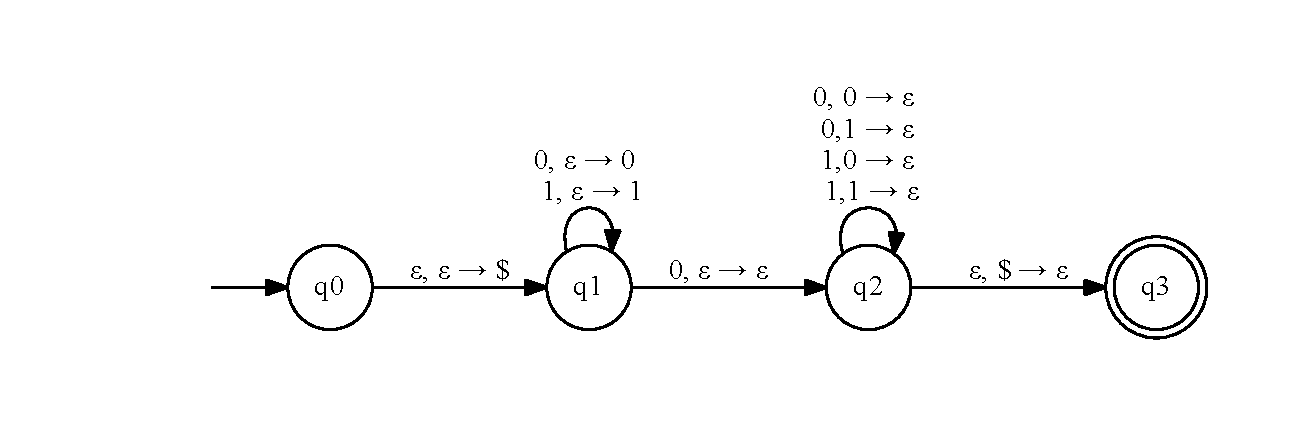
\includegraphics[width=0.8\textwidth]{d25.pdf}
\caption{The PDA for $L=\{w \mid$ the length of w is odd and its middle symbol is a 0 $\}.$}
\label{4}
\end{figure}
Brief Description: In this PDA we mark the bottom of the stack with a \$ then we non-deterministicly guess to loop or transition. If we loop we see a zero and push a zero,or we see an one and push an one. If we transition on a zero we pop and push nothing to the stack. Then we loop when we see a zero we either pop a zero or an one, or if we see an one we pop a zero or an one in either case we push nothing to the stack. Then we transition when the stack only has a \$ and we pop the \$ and accept.  \\
(e.)
\begin{figure}[H]
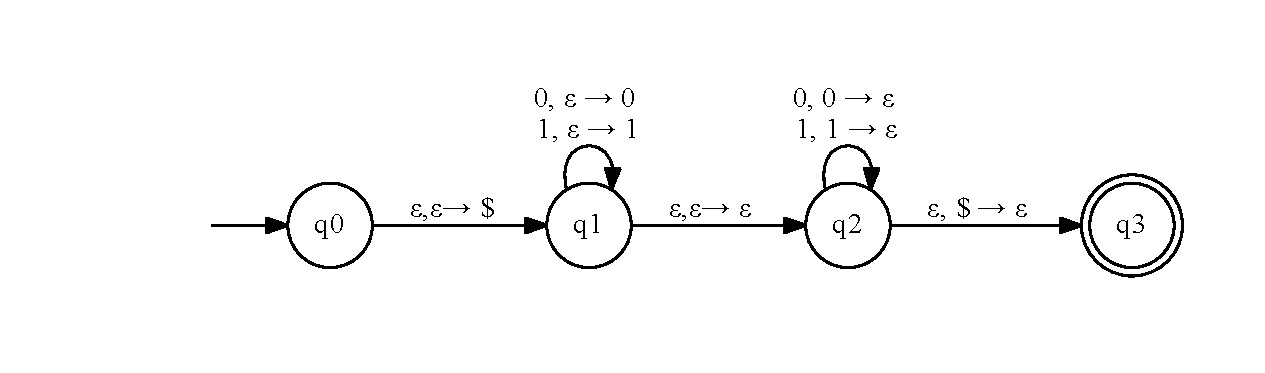
\includegraphics[width=0.8\textwidth]{e25.pdf}
\caption{The PDA for $L=\{w \mid w=w^R$,that is, w is a palindrome$\}.$}
\label{5}
\end{figure}
Brief Description:In this PDA  we mark the stack with a \$. Then we non-deterministicly guess. In the case we loop we do not pop anything from the stack, but we push a zero to the stack if we see a zero, or we push an one to the stack if we see an one. If we transition  on $\varepsilon$ we pop nothing and push nothing on the stack. Then we loop and on seeing a zero we pop a zero from the stack and push nothing. Likewise, we see an one we pop an one and push nothing until the stack has only a \$. Then we pop a \$ and accept. \\
(f.)
\begin{figure}[H]
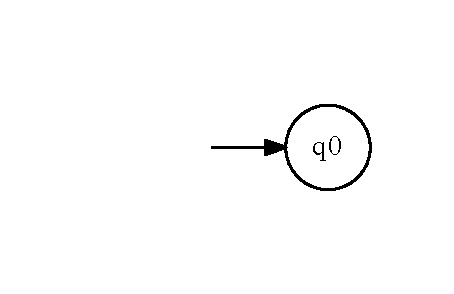
\includegraphics[width=0.5\textwidth]{f25.pdf}
\caption{The PDA for the empty set.}
\label{6}
\end{figure}
Brief Description: This PDA is a single not accepting state with no transitions.
\item[2.7]
(a.)
1.We mark the stack with an \$.\\
2.The PDA scans across the input.\\
3.If the PDA sees a b and its top stack symbol is a, it pops the stack.\\
4. If it scans a and its top stack symbol is a b, it pops the stack.\\
5.In all other cases, it pushes the input symbol onto the stack.\\
6.After the PDA finishes the input, if a is on top of the stack we pop the \$ and accepts. Otherwise do not accept.\\
(c.)
1.We mark the stack with an \$.\\
2.The PDA scans across the input string and pushes every symbol it reads until it reads a \#.\\
3.If \# is never read, do not accept.\\
4.Then the PDA skips over part of the input, nondeterminstically deciding when to stop skipping.\\
5.At that point, it compares the next input that finishes while the stack is nonempty, this branch of the PDA does not accept.\\
6.After the PDA finishes the input, if the stack becomes empty, the machine reads the rest of the input, then pops the \$ and accepts. \\
(d.)
1.We mark the stack with an \$.\\
2.The PDA scans across the input string and pushes every symbol it reads until it reads a \#\\
3.If a \# is never encountered we do not accept\\
4.After the PDA finishes input, if the stack becomes empty, the machine reads the rest of the input pops a \$ and accepts.
\item[2.10]
1.Nondeterministically break into two branches with each branch marking the stack with a \$.\\
2.Branch 1.\\
a.Read and push a's.\\
b.Nondeterministically guess when the first b is read
and begin popping symbols from the stack for each b read.\\
c.Then when there are not anymore symbols in the stack pop the \$ \\
d. See any numbers of c's and do not modify the stack and accept. Otherwise we do not accept.\\
3.Branch 2.\\
a.See a's do not modify the stack.\\
b.Nondeterministically guess when the first
b is read and begin pushing symbols on the stack for each b read.\\
c.Nondeterministically
guess when the first c is read, begin popping symbols from the stack for each c read.\\
d.When the stack empties precisely when the input string is done pop the \$ and accept.
\item[2.11]
\begin{figure}[H]
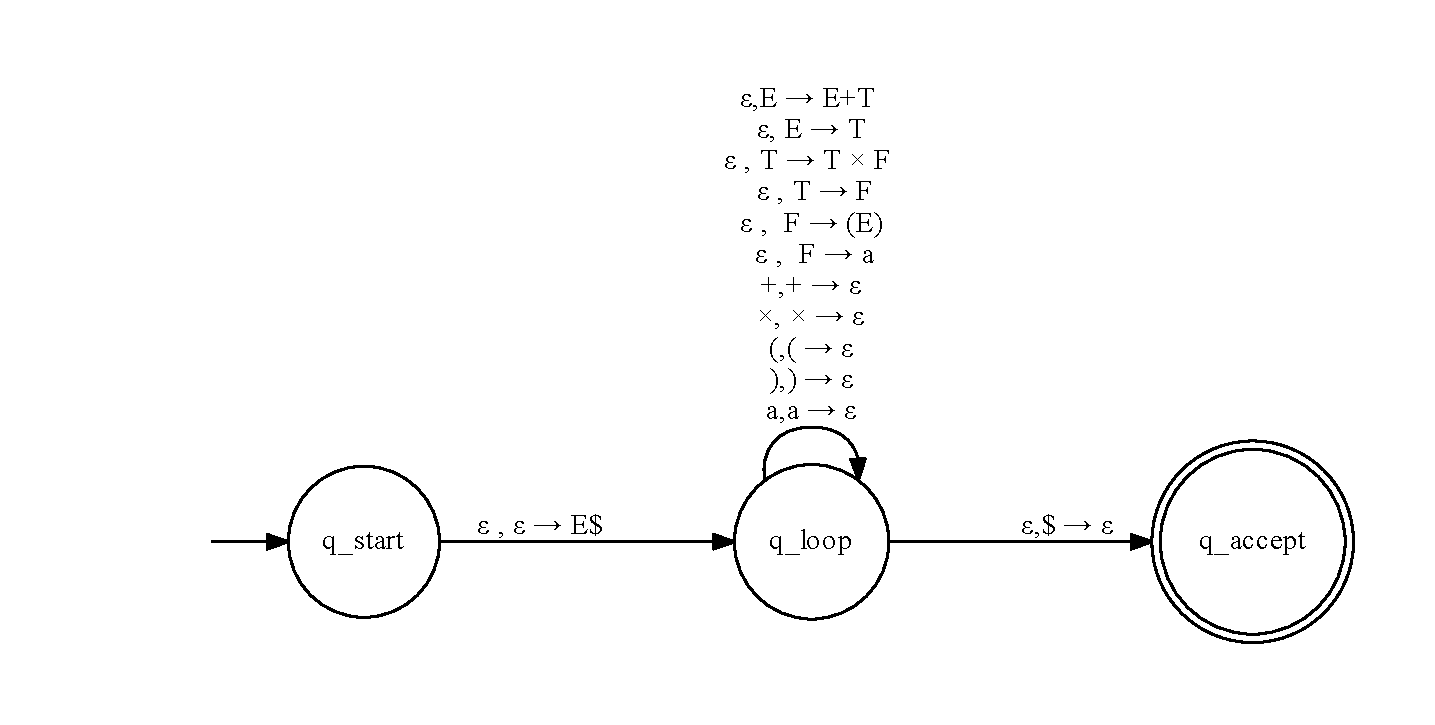
\includegraphics[width=0.9\textwidth]{a211.pdf}
\caption{The PDA for the CFG given in exercise 2.1.}
\label{7}
\end{figure}
\item[2.12]
\begin{figure}[H]
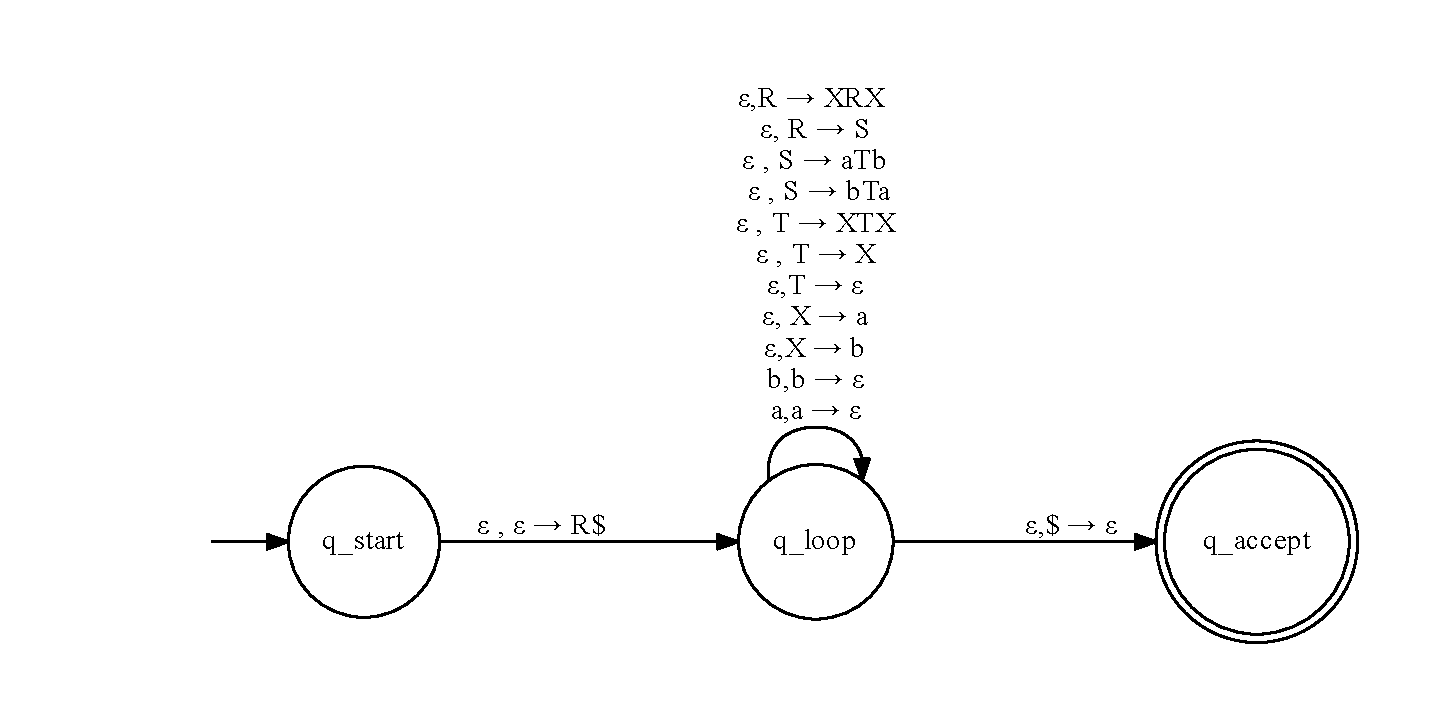
\includegraphics[width=0.9\textwidth]{a12.pdf}
\caption{The PDA for the CFG given in exercise 2.3.}
\label{8}
\end{figure}
\item[2.16]
\begin{proof}
Let $L_1$ and $L_2$ be CFLs. Their corresponding CFGs are $G_1$ and $G_2$ with start symbols $S_1$ and $S_2$.
(a.)Union:\\
$L_1 \cup L_2$ the CFG could be derived as follows:\\
$S \rightarrow S_1 \mid S_2$.\\
We go to either the start variable of $G_1$, which derives a string in $G_1$, or to the start variable of $G_2$ which derives a string in $G_2$.\\
(b.)Concatenation:\\
$L_1 L_2$ the CFG could be derived as follows:\\
$S \rightarrow S_1S_2$.\\
We derive something in $G_1$ followed by something in $G_2$.\\
(c.)Star
$L_1^{*}$ the CFG could be derived as follows:\\
$S \rightarrow SS_1 \mid \varepsilon$.\\
We derive the concatenation of one or more strings in $G_1$, or $\varepsilon$.
\end{proof}
\item[2.17]
\begin{proof}
Let R be a regular expression, then it can only be on one of six forms:\\
1.a for some a in the alphabet $\Sigma$:\\
2.$\varepsilon$\\
3.$\emptyset$\\
4.$(R_1 \cup R_2)$ where $R_1$ and $R_2$ are regular expressions. \\
5.$(R_1R_2)$where $R_1$ and $R_2$ are regular expressions.\\
6.$R_1^*$where $R_1$ is a regular expression.\\
Now let T,A, and B be variables in a CFG, then the types above will be produced as follows:\\
1.T $\rightarrow$ a for some a in the alphabet $\Sigma$.\\
2.T $\rightarrow \varepsilon$.\\
3.$T \rightarrow T$\\
4.T $\rightarrow$ A $\mid$ B\\
A $\rightarrow R_1$\\
B $\rightarrow R_2$\\
where $R_1$ and $R_2$ are regular expressions.\\ 
5.T $\rightarrow$ AB\\
A $\rightarrow R_1$\\
B $\rightarrow R_2$\\
where $R_1$ and $R_2$ are regular expressions.\\ 
6.T $\rightarrow$ AT $\mid \varepsilon$\\
A $\rightarrow R_1$\\
where $R_1$ is a  regular expression.\\ 
Thus, every regular expression is context free.
\end{proof}
\end{enumerate}
\end{document}